%%
%  ******************************************************************************
%  * #file    Szablon_raportu_EN_Latex.tex
%  * #author  Adrian Wójcik   adrian.wojcik(at)put.poznan.pl
%  *          
%  * #commit  Patryk Kościk   koscikpatryk(at)gmail.com
%  *          Modified the template for Projekt przejsciowy purposes          
%  *          
%  *
%  * #commit  Patryk Kościk   koscikpatryk(at)gmail.com
%  *          Zupełnie przewrócono na łeb formatke po taktycznym wyjasnieniu          
%  *          
%  * #version 1.1
%  * #date    09-Mar-2022
%  * #brief   PROJPRZEJ
%  *
%  ******************************************************************************
%%  
\documentclass[11pt, a4paper]{article}

\usepackage{SM_template}

% Wypełnijcie te dyrektywy zgodnie z waszym tematem
%
% \lab      -> NAZWA CZUJNIKA,          np.: 'DHT22'
% \comment  -> Króciutki opis co to,    np.: 'Cyfrowy czujnik temperatury'
% \author   -> Autor dokumentu          np.: Patryk Kościk
%
% Pamiętajcie o zmianie ścieżki w \addbibresourcue (!)

\lab{Suplement \#1}
\comment{Konfiguracja trybów GPIO}

%
% Początek dokumentu
%
\begin{document}

%
% Strona tytułowa
%
\mainpagenoimage

\newpage

\section* {Czujniki typu Digital Output}

Połączenie czujników typu DO wymaga skonfigurowania wybranego/wybranych pinów \textbf{GPIO} w trybie
\texttt{GPIO\_Input}.

\subsection*{Konfiguracja IOC}

Przechodzimy do zakładki GPIO:
\begin{figure}[h!]
    \centering
    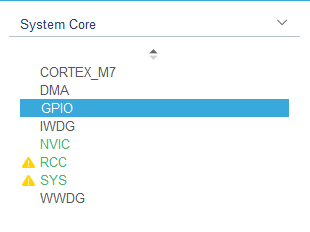
\includegraphics[width=0.6\textwidth]{IMAGES/gpio.png}
    \caption{Wybór zakładki GPIO}
\end{figure}

Przed wybraniem pinu należy sprawdzić w dokumentacji (REF), należy sprawdzić jakie stany logiczne (3.3V, 5V)
są obsługiwane. 
\begin{figure}[h!]
    \centering
    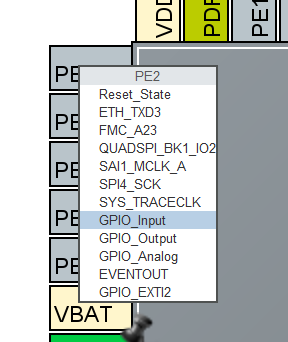
\includegraphics[width=0.4\textwidth]{IMAGES/input.png}
    \caption{Ustawienie pinu w tryb \texttt{GPIO\_Input}}
\end{figure}

\newpage

W następującym panelu możemy dodatkowo wybrać tryb podciągnięcia do masy lub napięcia $V_{cc}$.
Dostępna jest również opcja konfiguracji nazwy pinu, propagująca się do makrodefinicji w plikach \texttt{.c/h}:
\begin{figure}[h!]
    \centering
    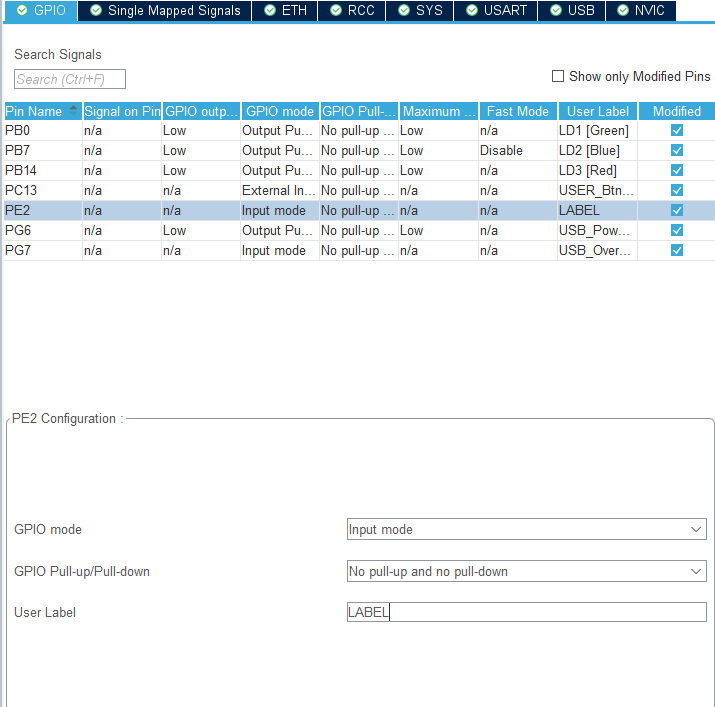
\includegraphics[width=0.6\textwidth]{IMAGES/input_konf.png}
    \caption{Panel konfiguracyjny GPIO}
\end{figure}

\subsection* {Tabela połączeń z mikrokontrolerem}
Po przeprowadzeniu konfiguracji przyjmujemy następujący przykładowy schemat połączeń:

\vspace{0.5cm}
\begin{table}[h!]
    \centering
    \begin{tabular}{|c|c|c|c|} 
        \hline
        \multicolumn{2}{|c|}{NUCELO-F746ZG} & \multicolumn{2}{c|}{SENSOR}   \\ 
        \hline
        Etykieta & Port i numer pinu        & Nr pinu & Etykieta            \\ 
        \hline
        GND     & -                         & 1       & -                   \\
        5V      & -                         & 2       &                     \\
        D7      & PF13                      & 3       & S                   \\
        \hline
    \end{tabular}
    \caption{Tabela połączeń czujnika z mikrokontrolerem. Pin oraz port zależy od konfiguracji pliku IOC}
\end{table}
\vspace{0.5cm}

Powyższa konfiguracja może być zastosowana między innymi dla czujników:

\begin{itemize}
    \item Czujnik przechylenia
    \item Czujnik stuknięć
    \item Kontaktron
    \item Przechylenia rtęciowy
    \item Dotyku
    \item Płomienia
\end{itemize}

\subsection* {Kod obsługujący odczyt z czujnika}
\begin{lstlisting}[style=lstC, caption={Kod pętli \texttt{while()}}]
if (HAL_GPIO_ReadPin(PF13_GPIO_Port, PF13_Pin))
{
    /* sygnał odebrany */
    HAL_GPIO_WritePin(LD1_GPIO_Port, LD1_GPIO_Pin, 1);
}
else
{
    /* brak sygnału */
    HAL_GPIO_WritePin(LD1_GPIO_Port, LD1_GPIO_Pin, 0);
}

HAL_DELAY(100);
\end{lstlisting}

\newpage





\section* {Aktuatory typu Digital Input}

Połączenie czujników typu DI wymaga skonfigurowania wybranego/wybranych pinów \textbf{GPIO} w trybie
\texttt{GPIO\_Output}.

\subsection*{Konfiguracja IOC}

Przechodzimy do zakładki GPIO:
\begin{figure}[h!]
    \centering
    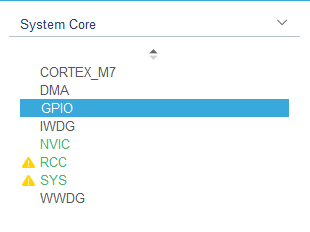
\includegraphics[width=0.6\textwidth]{IMAGES/gpio.png}
    \caption{Wybór zakładki GPIO}
\end{figure}

Przed wybraniem pinu należy sprawdzić w dokumentacji (REF), należy sprawdzić jakie stany logiczne (3.3V, 5V)
są obsługiwane. 
\begin{figure}[h!]
    \centering
    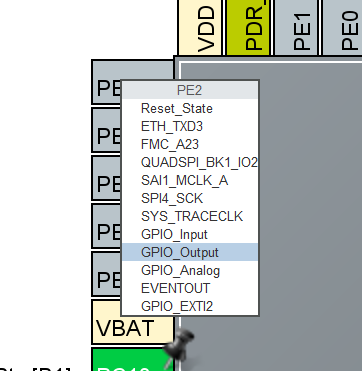
\includegraphics[width=0.4\textwidth]{IMAGES/output.png}
    \caption{Ustawienie pinu w tryb \texttt{GPIO\_Output}}
\end{figure}

\newpage

W następującym panelu możemy dodatkowo wybrać tryb podciągnięcia do masy lub napięcia $V_{cc}$, oraz parametr
\texttt{Maximum output speed}.
Dostępna jest również opcja konfiguracji nazwy pinu, propagująca się do makrodefinicji w plikach \texttt{.c/h}:
\begin{figure}[h!]
    \centering
    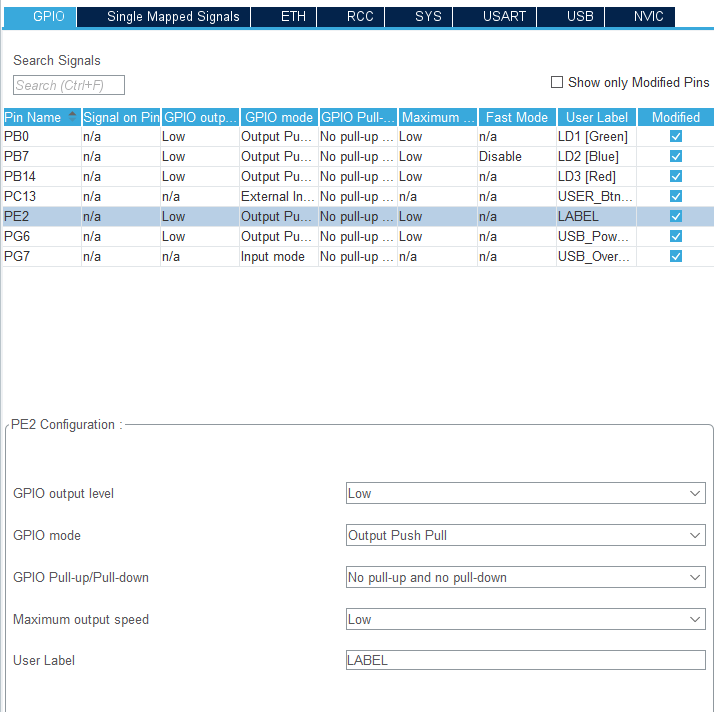
\includegraphics[width=0.6\textwidth]{IMAGES/output_konf.png}
    \caption{Panel konfiguracyjny GPIO}
\end{figure}

\subsection* {Tabela połączeń z mikrokontrolerem}
Po przeprowadzeniu konfiguracji przyjmujemy następujący przykładowy schemat połączeń:

\vspace{0.5cm}
\begin{table}[h!]
    \centering
    \begin{tabular}{|c|c|c|c|} 
        \hline
        \multicolumn{2}{|c|}{NUCELO-F746ZG} & \multicolumn{2}{c|}{SENSOR}   \\ 
        \hline
        Etykieta & Port i numer pinu        & Nr pinu & Etykieta            \\ 
        \hline
        GND     & -                         & 1       & -                   \\
        5V      & -                         & 2       &                     \\
        D7      & PF13                      & 3       & S                   \\
        \hline
    \end{tabular}
    \caption{Tabela połączeń czujnika z mikrokontrolerem. Pin oraz port zależy od konfiguracji pliku IOC}
\end{table}
\vspace{0.5cm}

Powyższa konfiguracja może być zastosowana między innymi dla aktuatorów:

\begin{itemize}
    \item Buzzer aktywny/pasywny
    \item Przekaźnik
    \item Laser
\end{itemize}

\subsection* {Kod obsługujący aktuator}
\begin{lstlisting}[style=lstC, caption={Kod pętli \texttt{while()}}]
if (HAL_GPIO_ReadPin(USER_BUTTON_Port, USER_BUTTON_Pin))
{
    /* ustawienie sygnału wyjścia */
    HAL_GPIO_WritePin(LABEL_Port, LABEL_GPIO_Pin, 1);
}
else
{
    /* brak sygnału */
    HAL_GPIO_WritePin(LABEL_Port, LABEL_GPIO_Pin, 0);
}

HAL_DELAY(100);
\end{lstlisting}





\newpage


\section* {Wyjście PWM}

Aby uruchomić i sterować wyjście PWM należy najpierw uruchomić \texttt{timer}:

\subsection*{Konfiguracja timera}

\begin{figure}[h!]
    \centering
    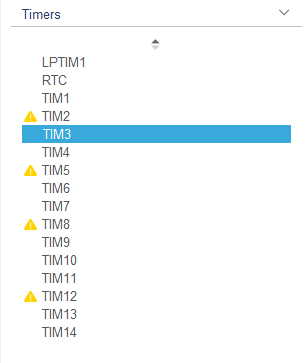
\includegraphics[width=0.3\textwidth]{IMAGES/tim.png}
    \caption{Zakładka Timers}
\end{figure}

Po wybraniu układu (np. TIM3), ujrzymy zakładkę konfiguracyjną: 
\begin{figure}[h!]
    \centering
    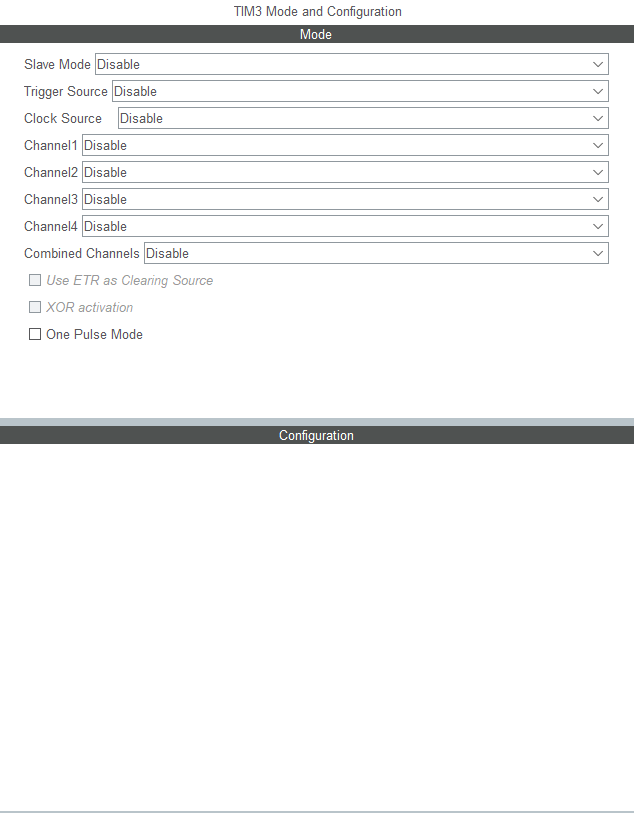
\includegraphics[width=0.5\textwidth]{IMAGES/tim_empty.png}
    \caption{Panel konfiguracyjny GPIO}
\end{figure}

\newpage

Następnie należy ustawić \texttt{Clock Source} na \texttt{Internal clock}

\begin{figure}[h!]
    \centering
    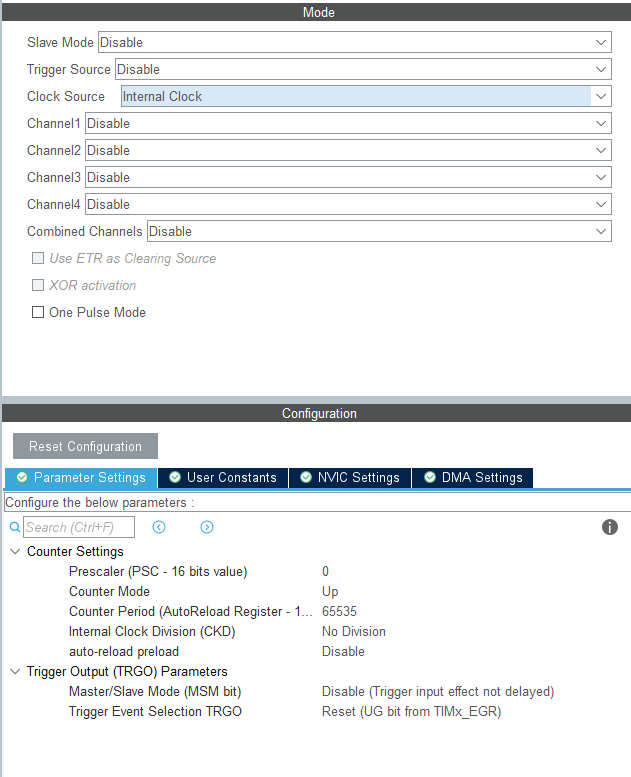
\includegraphics[width=0.6\textwidth]{IMAGES/tim_timer.png}
    \caption{Panel konfiguracyjny GPIO}
\end{figure}

W tym momencie timer jest skonfigurowany. Jego częstotliwość wyzwoleń (zliczania) jest konfigurowana poprzez
parametry:

\begin{itemize}
    \item Prescaler (PSC)
    \item Couter Period (ARR)
    \item Internal clock division (CDK)
\end{itemize}

oraz opisana wzorem:

\[
f_{clk} = \frac{f_{cpu}}{(PSC+1)\cdot(ARR+1)\cdot(CDK+1)}
\]

\vspace{0.5cm}
Aby uruchomić wsparcie przerwań, należy włączyć \texttt{NVIC}:
\begin{figure}[h!]
    \centering
    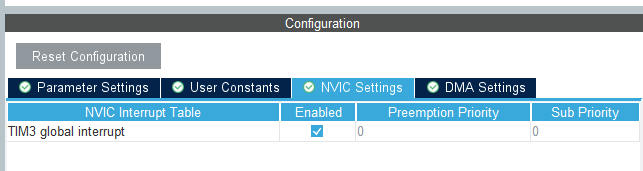
\includegraphics[width=0.4\textwidth]{IMAGES/tim_nvic.png}
    \caption{Zakładka NVIC}
\end{figure}


\newpage

\subsection*{Konfiguracja PWM}

Aby skonfigurować PWM należy wybrać opcje \texttt{PWM Out}:

\begin{figure}[h!]
    \centering
    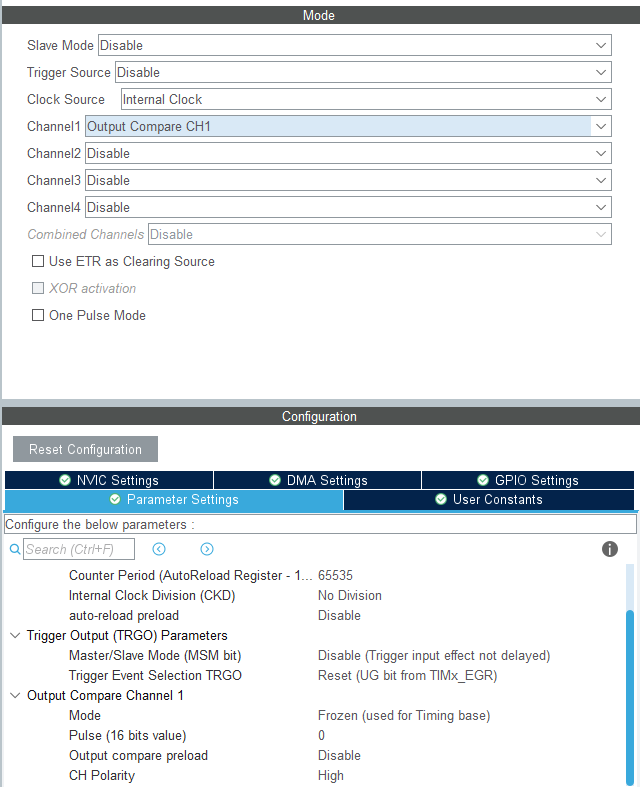
\includegraphics[width=0.6\textwidth]{IMAGES/tim_pwm_konf.png}
    \caption{Uruchomienie wyjścia PWM}
\end{figure}

STM32CubeIDE wybierze nam domyślnie pin, który możemy podejrzeć w zakładce GPIO:

\begin{figure}[h!]
    \centering
    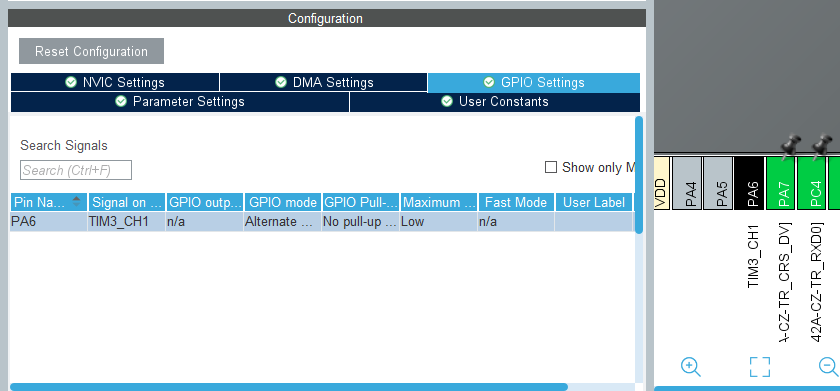
\includegraphics[width=0.6\textwidth]{IMAGES/tim_pwm_pin.png}
    \caption{Zakładka GPIO dla PWM}
\end{figure}

\newpage

\subsection* {Kod obsługujący PWM}
\begin{lstlisting}[style=lstC]

//Autowygenerowane:
MX_TIM3_Init();

// Uruchamiamy TIM w trybie PWM
HAL_TIM_PWM_Start(&htim3, TIM_CHANNEL_1);

// Deklarujemy zmienną wypełnienia
int i = 0;

// Pętla while(1)
if(i < 100)
{
    __HAL_TIM_SET_COMPARE(&tim3, TIM_CHANNEL_1, i*100);
    i++;
}
else
{
    i = 0;
}

HAL_DELAY(100);
\end{lstlisting}



\end{document}